\section{Identifikation der Parameter}
\label{sec.Parameter}

Das im Theorieteil betrachtete Modell des Furuta-Pendels (siehe \cite{Cazzolato.2011}) unterscheidet sich von dem Modell des zu verwendenden Furuta-Pendels des Institutes, wie in Abbildung~\ref{fig.FurutaPlant} ersichtlich.
Die gegeben bzw. gemessenen Parameter müssen daher an das theoretische Modell angepasst werden. Für die Längen der Pendelarme gilt somit:

\begin{figure}[htbp]
	\centering
	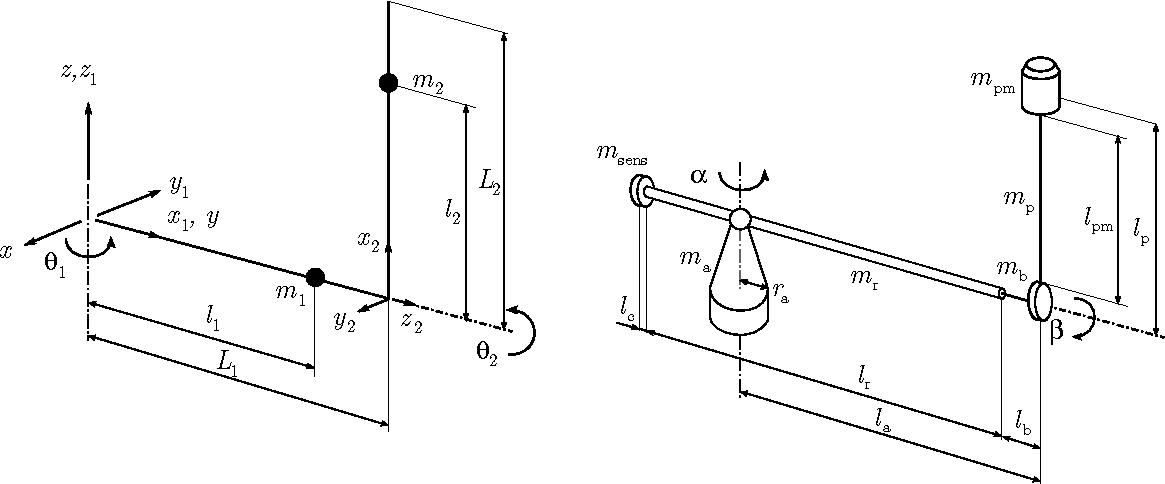
\includegraphics[width=1.\textwidth]{Grafiken/adelaideimagenew}
	\caption{Darstellung des Furuta-Pendels. (Zur Verfügung gestellt vom Betreuer des Labors) }
	\label{fig.FurutaPlant}
\end{figure}

Die gegeben bzw. gemessenen Parameter müssen daher an das theoretische Modell angepasst werden. Für die Längen der Pendelarme gilt somit:

\begin{eqnarray}
L_1 &=& l_a \nonumber \\
L_2 &=& l_{pm} \nonumber 
\end{eqnarray}

Zusätzlich lässt sich der Abstand des Sensors von der Drehachse um $\theta_1$  wie folgt berechnen:

\begin{equation}
l_{sens} = l_r+l_b-l_a+\dfrac{l_c2}{2}
\end{equation}

Die Punktmassen des theoretischen Pendel-Modells ergeben sich bei Beachtung der Trägheitsachsen zu:
\begin{eqnarray}
m_1 &=& m_{sens}+m_r+m_a \nonumber \\
m_2 &=& m_p+m_{pm}
\end{eqnarray}

Die Massenträgheiten können ebenso zusammengefasst werden und ergeben sich wie folgt:
%Kai: ich habe einfach unsere equations aus matlab eingefügt!
%Thomas: ja, das merkt man ^^ hier ist gan
\begin{eqnarray*}
J_{1,norm}&=&\dfrac{J_M +J_{Enc,1}+(m_r \cdot l_r \cdot l_r)}{12+(m_r (-0.5 l_r-l_b+l_a)^2)+(\dfrac{4}{10}) (m_a  {r_a}^{2})} \\
J_{2,norm}&=& J_{m,b}+J_{Enc2}   + \dfrac{(m_p \cdot {l_p}^{2})}{3} \\
J_0&=&J_{1,norm}+ m_1 \cdot {l_1}^{2} + m_2 \cdot {L_1}^{2} \\ 
J_2&=&J_{2,norm}+m_2 \cdot {l_2}^2           \\
\end{eqnarray*}

Für die Längen $l_1$ und $l_2$ erhält man
\begin{align*}
l_1 &= \sqrt{\frac{(l_{sens}^2 \dot m_{sens}+l_b^2 \dot m_b)}{m_{sens} + m_b})} \\
l_2 &\cong l_{pm}
\end{align*}

%Kai: ab hier sind das wieder die von dustin/den anderen!
und für die einzelnen Trägheitsmomente:
\begin{align*}
J_{arm} &= m_r \frac{l^2_r}{12}+m_r(\frac{1}{2}l_r+l_b-l_a)^2 \\
J_{pend,1} &= m_bl^2_a \\
J_{sens} &= m_{sens}(l_a-l_b-l_r-\frac{1}{2}l_c)^2 \\
J_{ps} &= m_p(r_b+\frac{1}{2}l_p)^2 \\
J_{pm} &= m_{pm}l^2_{pm} \\
J_{arm}+J_{pend1}+J_{sens} &= m_1l^2_1 \\ 
J_{pm}+J_{ps} &= m_2l^2_2 \\
\end{align*}

%Hier sind unsere werte! noch viele Latex-Fehler!
% Thomas: ich schreib hier mal einen Absatz.
Die folgenden Werte sind im Zuge des Labors zu Verfügung gestellt oder durch rudimentäre Messungen erhalten und werden an dieser Stelle der Vollständigkeit halber aufgeführt. 
\begin{align*}
b_1 &= \SI{1e-4}{\newton\metre\second} &
b_2 &= \SI{2.8e-4}{\newton\metre\second} \\
g &= \SI{9.81}{\metre\per\square\second} &
k_{1,phi} &= \SI{0.5}{}\\
R_a &= \SI{10}{\ohm} &
J_M  &=  \SI{6.75e-6}{\kilo\gram\square\metre}  \\        % Inertia Motor 6.75e-6
J_{Enc1}  &=  \SI{6e-14}{\kilo\gram\square\metre}  &        % Inertia Encoder Theta1
J_{Enc2}  &=  \SI{0.1e-6}{\kilo\gram\square\metre}  \\     % Inertia Encoder Theta2
J_{m,b}  &=  \SI{3.98125e-6}{\kilo\gram\square\metre}  &     % Inertia m_b
m_{sens}  &=  \SI{0.084}{\kilo\gram}  \\
l_c  &=  \SI{0.01}{\metre}  &
m_{horzArm} &= \SI{0.284}{\metre} \\
m_b &= \SI{0.025}{\metre}  &
m_a &= \SI{0.190}{\metre} \\
r_a &= \SI{0.015}{\metre}  &
r_b &= \SI{0.0176}{\metre} \\
l_r &= \SI{0.29}{\metre} &
m_r  &=  m_{horzArm} - m_{sens}\\
l_a &= \SI{.175}{\metre} &
l_b &= \SI{.01}{\metre}\\
m_{pm} &= \SI{0.0379}{\kilo\gram} &
m_p &= \SI{0.0157}{\kilo\gram}\\
l_{pm} &= \SI{0.229}{\metre} &
l_p &= \SI{0.262}{\metre}\\
\end{align*}

Die Gleichung des DC-Motors, der den Pendelarm und somit direkt $\theta_2$ antreibt, kann aus dem Research Articles der University of Adelaide, entnommen werden \citep{Cazzolato.2011}:

\begin{equation}
V = L_m \cdot \dot{i} + R_m \cdot i + K_m \cdot \theta_1
\end{equation}

Umgestellt nach $ \dot{i}$ ergibt sich folgende Gleichung:

\begin{equation}
 \dot{i} = \dfrac{V \cdot R_m \cdot i - K_m \cdot \dot{\theta_1}}{L_m}
\end{equation}

Für das Drehmoment des Motors gilt:
\begin{equation}
\tau = K_m \cdot i 
\end{equation}

Auch die Parameter des DC-Motors wurden aus dem Dokument entnommen. Folgende Parameter sind gegeben:

\begin{align}
K_m &= 0,09 ~\dfrac{Nm}{A} \\
R_m &= 7,8  ~\Omega \\
L_m &= 0,005  ~H 
\end{align}
